\graphicspath{{./chapters/ncov-escape/}}
\chapter{Forecasting SARS-CoV-2 lineage success from molecular data}

In this chapter, we develop and discuss methods for predicting relative fitness using molecular data.
We intend to expand this chapter into a larger paper.
This expanded paper will include analyses on how long the predictive power of molecular data lasts as well as more replicates of this idea for evolution post-BA.2 and post-JN.1.

\section{Abstract}

% Most methods are statistical.
% Though some theoretical work has been done to understand how mechanism informs relative fitness, there is still a need to build predictive model that can use data for this prediction.
%
% We develop methods for estimating and predicting relative fitness using evolutionary history and molecular data and leverage these methods to build models that enable out of sample prediction of relative fitness based on patterns of descent.
SARS-CoV-2 variants have driven global waves of infection, shifting from transmissibility-driven success in Alpha and Delta to immune escape in Omicron and its descendants.
Models estimating relative fitness from variant frequencies provide short-term insights but often fail in long-term forecasts due to dynamic fitness landscapes and neglect of evolutionary history.
Simulations reveal that this oversight inflates correlations between molecular phenotypes and fitness, misattributing patterns to ancestry rather than mechanism.
To address this, we introduce a Bayesian framework that integrates molecular phenotypes, such as immune escape and receptor binding, with phylogenetic structure.
By leveraging innovation-based regression priors, our method accounts for shared ancestry and fitness changes along lineages, enabling robust out-of-sample predictions.
This framework advances forecasting of SARS-CoV-2 variant success and offers a generalizable tool for understanding and responding to the evolution of rapidly mutating pathogens.

\section{Introduction}

The COVID-19 pandemic has been characterized by the emergence of SARS-CoV-2 variants that have driven successive waves of infection globally. %TODO: Bunch of citations
Early variants like Alpha, Beta, Gamma, and Delta achieved success largely through increases in intrinsic transmissibility.
However, the emergence of Omicron marked a shift towards immune escape became the dominant driver of variant success, as demonstrated by molecular studies showing reduced neutralization by vaccine and infection-derived immunity.

Subsequent Omicron-derived lineages, including XBB, EG.5.1, and JN.1, have further exploited immune escape to drive rapid turnover in the viral population.
This shift underscores the interplay between population immunity and variant fitness, where increasing exposure selects for variants with immune escape.
Understanding the molecular and evolutionary factors that shape the success of these variants is critical for anticipating outbreaks and guiding vaccine design.

Currently, efforts to predict the success of viral variants rely heavily on models that estimate relative fitness from changes in variant frequencies over time. \cite{Piantham2022, Figgins2021}.
These models, while valuable for short-term forecasting, often fail to generalize over longer time horizons due by repeated variant emergence or time-dependence in relative fitness \cite{abousamra2024fitness}.  
Theory predicts that relative fitness should be a function of both escape against particular immune backgrounds and the distribution of these backgrounds in the population (Chapter 4).
This suggests the improving forecasts of relative fitness will require integrating of molecular phenotypes to improve long-term forecasting capabilities.

Experimental methods such as neutralization titer assays and deep mutational scanning (DMS) provide valuable molecular estimates of immune escape.
Although they have correlations with population-level success, it remains unclear how these data can be used to predict variant success  \cite{Dadonaite2023}. % Cite Cao and Bloom
Protein language models (PLMs) have recently emerged as tools to infer molecular properties directly from sequences and have even been used to predict relative fitness. %TOOD: Ito paper?
However, both PLMs and traditional regression-based approaches share a critical weakness: they fail to account for the shared evolutionary history of variants. 
This oversight inflates correlations between molecular phenotypes and fitness, with shared ancestry rather than mechanistic relationships driving the observed patterns,

Using simulations, we show that naive tip-level regressions overestimate the strength of associations between molecular phenotypes and fitness due to recent shared evolutionary history.
In contrast, innovation-based approaches better isolate meaningful relationships between molecular phenotypes and fitness.
These findings highlight a key limitation in existing methods and suggest a need for evolutionarily-informed approaches.

To address these challenges, we introduce a Bayesian framework that integrates molecular phenotypes, such as immune escape and receptor binding, with phylogenetic structure to estimate and predict relative fitness.
By leveraging innovation-based regression priors, this method accounts for shared ancestry and fitness innovations between lineages, enabling out-of-sample predictions of relative fitness.

% Approaches using molecular and phylogeny-based features for longer-term frequency forecast have been used in influenza to varying levels of success \cite{huddleston2020integrating, luksza2014predictive}.
%
% %TODO: What is the difference here?
%
% Additionally, incorporation of external data for validation of estimated growth advantage has occurred.
%
% Despite the existence of molecular estimates of immune escape exist, there’s little work combining these for forecasting of variant success in the future.
%
% First, we show that escape scores and RBD ACE-2 binding computed from DMS are associated with higher growth advantages in emerging Pango lineages.
% We then combine existing data into a new model to jointly estimate variant growth advantages accounting for evolutionary relationships between viruses and enable prediction of new variants based on this phylogenetic structure.
% We also introduce a fully Bayesian model of variant growth advantages which incorporates both phylogenetic structure in its estimate to provide informed priors of a variant's relative fitness using molecular estimates of immune escape and its phylogenetic placement.
% We then apply this work to identify likely escape candidates from BA.2 derived immunity and repeat this analysis for XBB.1.5.

\section{Results}

The evolutionary success of SARS-CoV-2 lineages is influenced by a combination of molecular phenotype and population immunity.
The interplay between these factor creates challenges for accurately attributing changes in lineage frequency to specific phenotypic drivers, such as immune escape.
Recent shared evolutionary history additionally introduces confounding effects that can obscure relationships between molecular phenotypes and fitness, particularly when using naive regression approaches.
These challenges necessitate a framework capable of disentangling the direct contributions of molecular traits from the effects of evolutionary relatedness.

We provide an overview of the evolutionary and phenotypic context used to quantify and analyze fitness innovations in Fig.~\ref{fig:interplay_phylo_escape_fitness}.

The evolutionary relationships among SARS-CoV-2 clades are often visualized by Pango lineage and Nextstrain clade.
These variant groupings allow us to easily classify and enumerate genetic variation in the population, creating nested structure in Pango lineages and enabling us to visualize their variant-parent relationships.
These variant parent relationships reflect Nextstrain clades (Fig. \ref{fig:interplay_phylo_escape_fitness}A).
However, despite falling into the same clade, lineages may vary in their molecular phenotypes such receptor-binding domain (RBD) immune escape (Fig.~\ref{fig:interplay_phylo_escape_fitness}B). 

This phenotypic variation among lineages coexists with the temporal dynamics of selection in SARS-CoV-2.
Tracking the frequencies of Nextstrain clades from January to November 2023 shows the rapid turnover of clades driven by shifts in fitness among lineages (Fig.~\ref{fig:interplay_phylo_escape_fitness}C).

Naive regression methods show that these molecular phenotypes poorly explain relative fitness of variants ($R^2 = 0.03$), suggesting that molecular phenotypes may not be useful for predicting lineage success (Fig.~\ref{fig:interplay_phylo_escape_fitness}D).
However, accounting for evolutionary relationships using variant-parent innovation (Fig.~\ref{fig:interplay_phylo_escape_fitness}E) in relative fitness and phenotype reveal clearer signal ($R^2 = 0.69$).

By focusing on the changes along branches, we isolate the impact of molecular phenotypes from correlations due to shared evolutionary history.
These fitness innovations can be used to identify phenotypic drivers of relative fitness and to enable forecasting of relative fitness for yet unseen variants.
Together, these results provide insights into the mechanisms underlying lineage success and advance the ability to forecast the emergence of novel variants.

\begin{figure}[h]
    \centering
    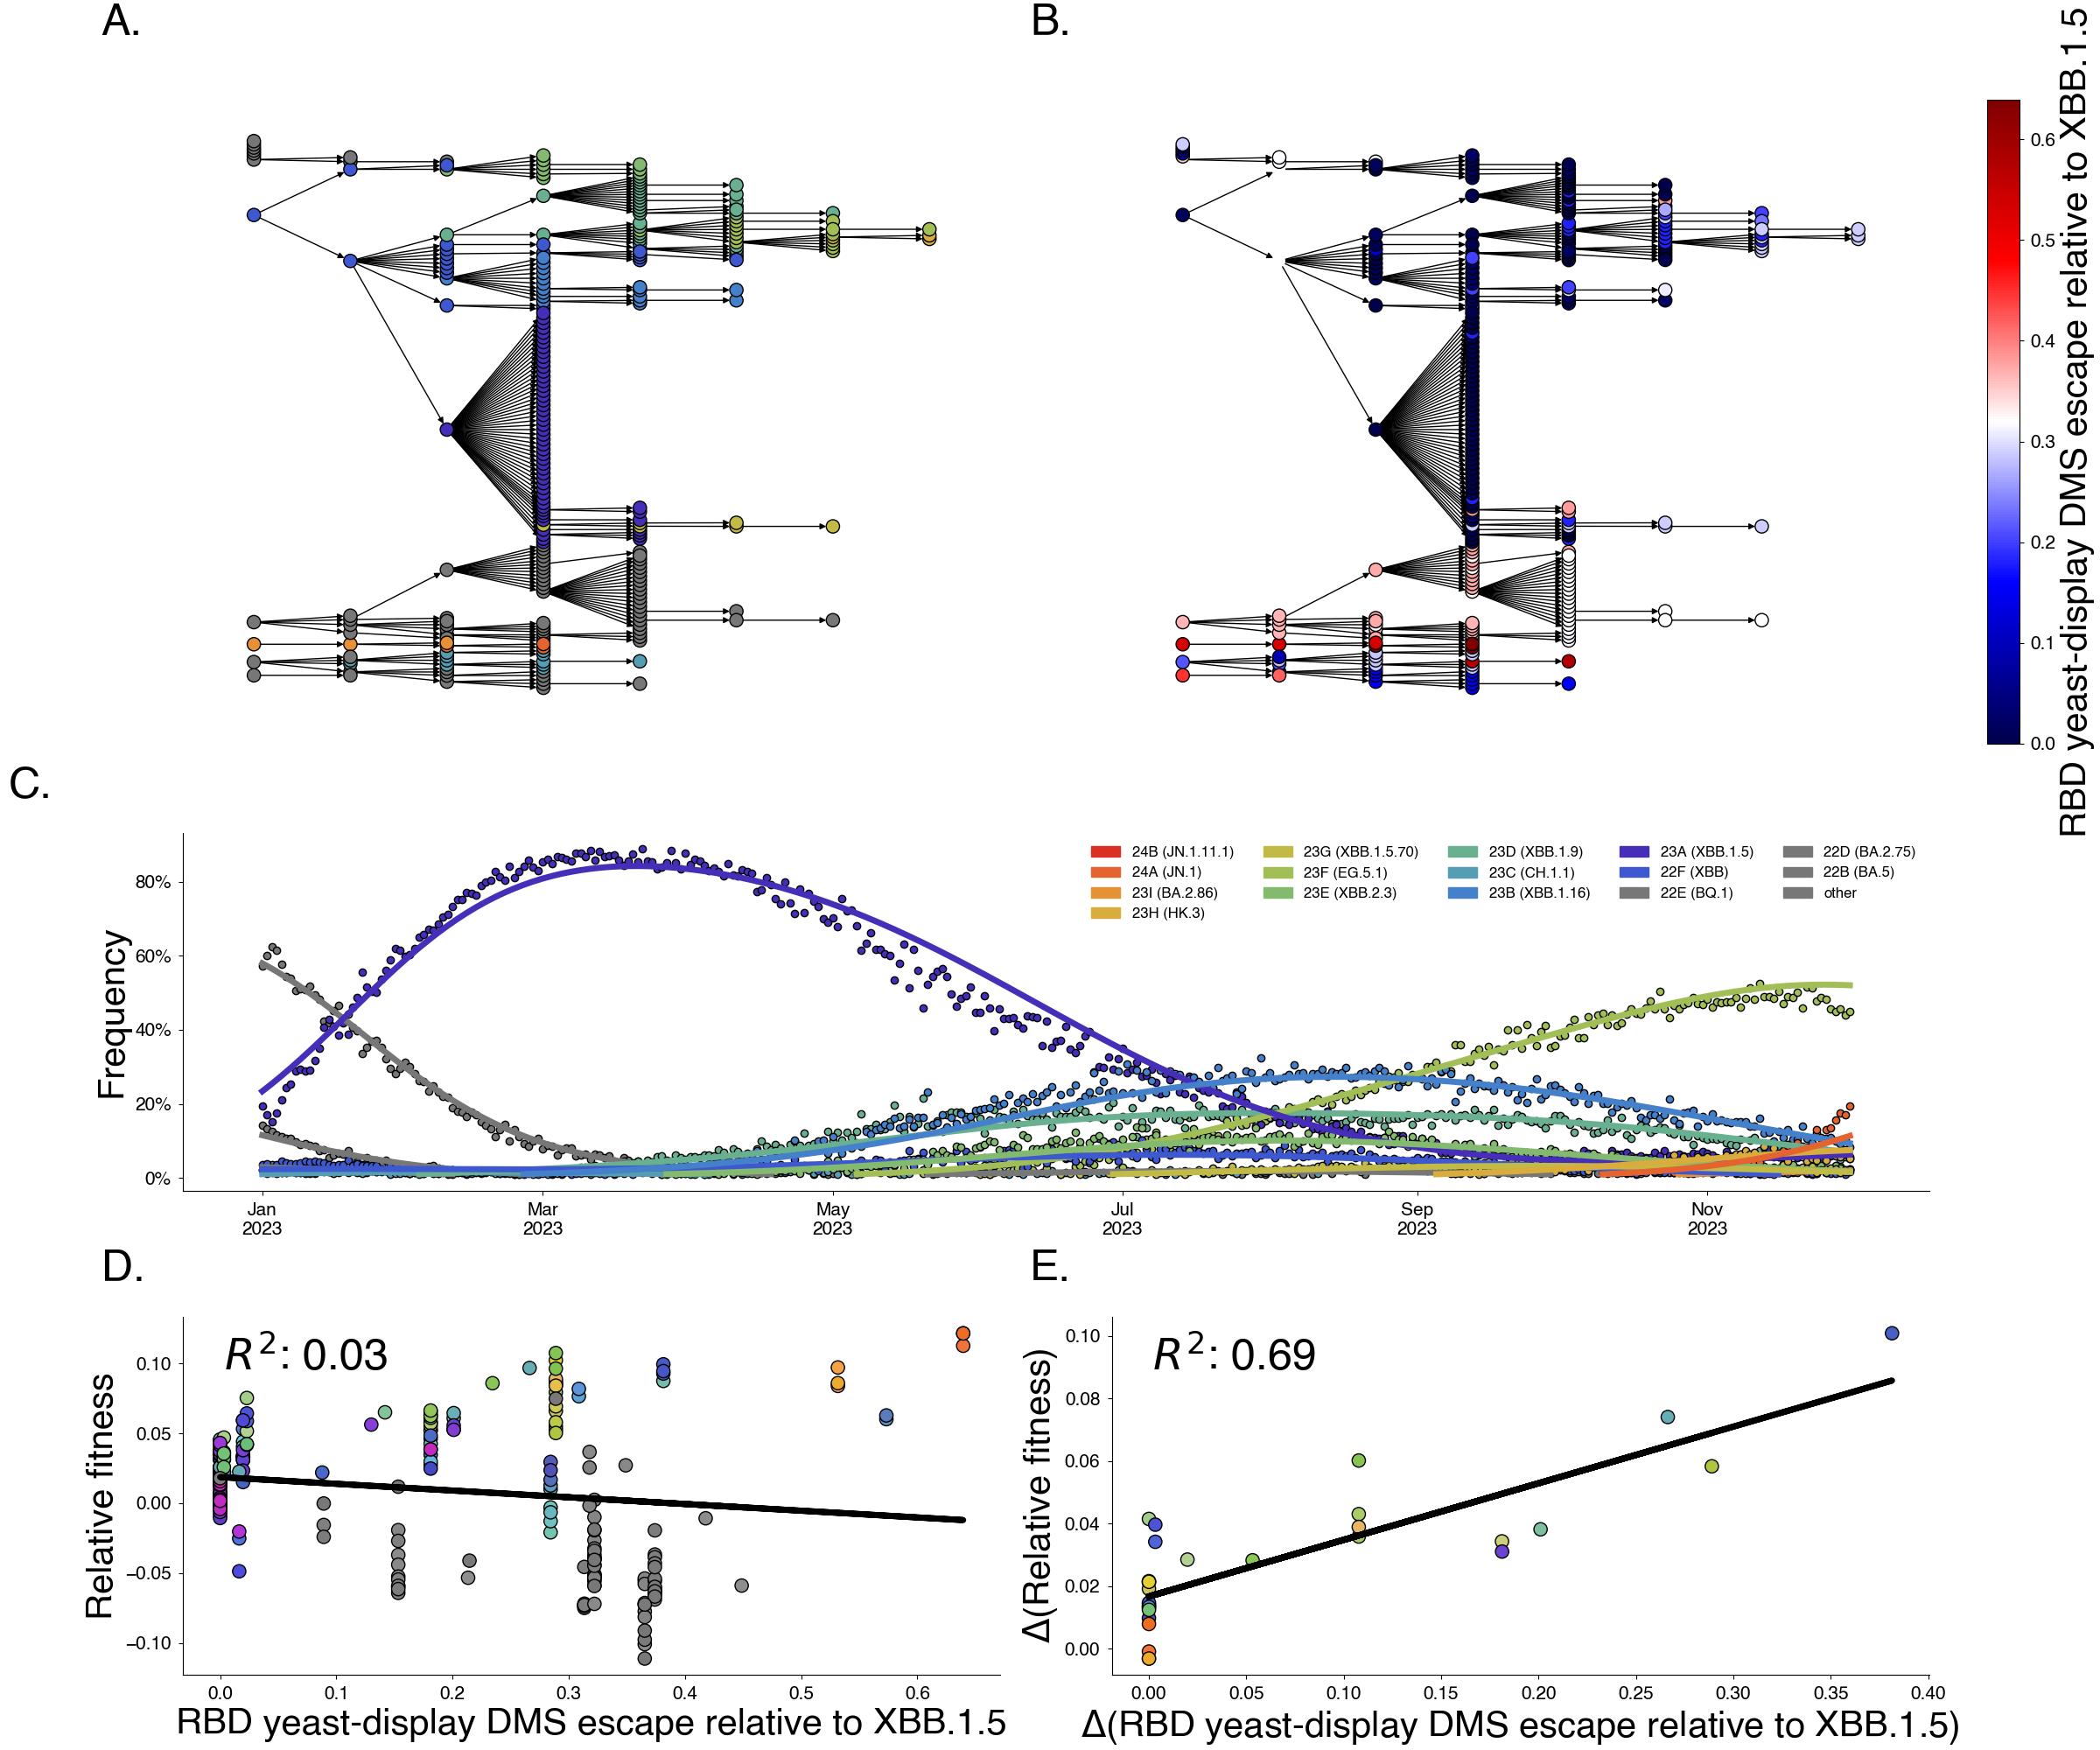
\includegraphics[width=0.9\textwidth]{./figures/interplay_phylo_escape_fitness.png}

    \caption[\textbf{Interplay between evolution, immune escape, and fitness among SARS-CoV-2 variants.}]{
	\textbf{Interplay between evolution, immune escape, and fitness among SARS-CoV-2 variants}
	A. Lineage and closest parent mapping of SARS-CoV-2 Pango lineages, with nodes colored by Nextsrain clade, illustrating evolutionary relationships and grouping of lineages.
	B. The mapping as A., now colored by receptor-binding domain (RBD) immune escape, highlighting molecular phenotypes across evolutionary lineages.
	C. Temporal dynamics of clade frequencies in the global SARS-CoV-2 population from January to November 2023. The figure highlights the rapid turnover of clades driven by changing fitness landscapes.
	D. Naive correlation between RBD immune escape (x-axis) and relative fitness (y-axis) shows weak association ($R^2 = 0.03$), reflecting the confounding effects of shared ancestry.
	E. Innovation-based correlation between immune escape contrasts and fitness innovations shows a significantly stronger relationship ($R^2 = 0.69$), demonstrating the importance of accounting for evolutionary context to uncover true mechanistic drivers of fitness.
    }
    \label{fig:interplay_phylo_escape_fitness}
\end{figure}

\paragraph{Shared evolutionary history generates spurious correlations}

In naive regression methods, cumulative molecular phenotypes, such as immune escape, are directly correlated with measures of fitness.
This naive approach often fails to account for the nested structure and shared evolutionary of lineages which can generate spurious correlations between fitness and phenotype in closely related lineages.

Simulating phylogenetic trees under selection, we show that fitness increases over time as more fit lineages reproduce in the population (Fig.~\ref{fig:shared_history_spurious_correlation}A).
Though we simulate this tree assuming selection is independent of individual mutations or their number, we find that the total number of mutations explains much of the variance in relative fitness ($R^2=0.76$), as shown in Fig.~\ref{fig:shared_history_spurious_correlation}B.
This spurious correlation is due to shared evolutionary history creating correlations between individual lineages in the population despite branch level innovations being independent.
In fact, we can see that the magnitude of the $R^2$ increases with the variation in fitness between branches i.e. the strength of selection in the population (Fig.~\ref{fig:fitness-variation-variance-explained}A).
This suggests that stronger selection amplifies the confounding effect of shared ancestry.

To address this challenge, we focus on fitness innovations i.e. branch-specific changes in relative fitness. 
Using innovations or changes in fitness and mutations across branches within our regressions, we isolate the contributions of molecular phenotypes to fitness, effectively removing the confounding effects of shared ancestry (Fig.~\ref{fig:shared_history_spurious_correlation}C).
This relationship between fitness innovations and mutation change is preserved across varying levels of selection strength (Fig.~\ref{fig:fitness-variation-variance-explained}B).

We show that this approach is similar to other approaches of dealing with confounding due to shared ancestry such as phylogenetic generalized least squares in Supplementary Text~\ref{ssec:pgls}.

Using innovations enables us to better resolve drivers of fitness that are obscured by recent evolutionary history.
By isolating the contributions of molecular phenotypes to fitness, this provides a robust foundation for identifying the specific drivers of relative fitness and improving predictions of lineage success.

\begin{figure}[h]
    \centering
    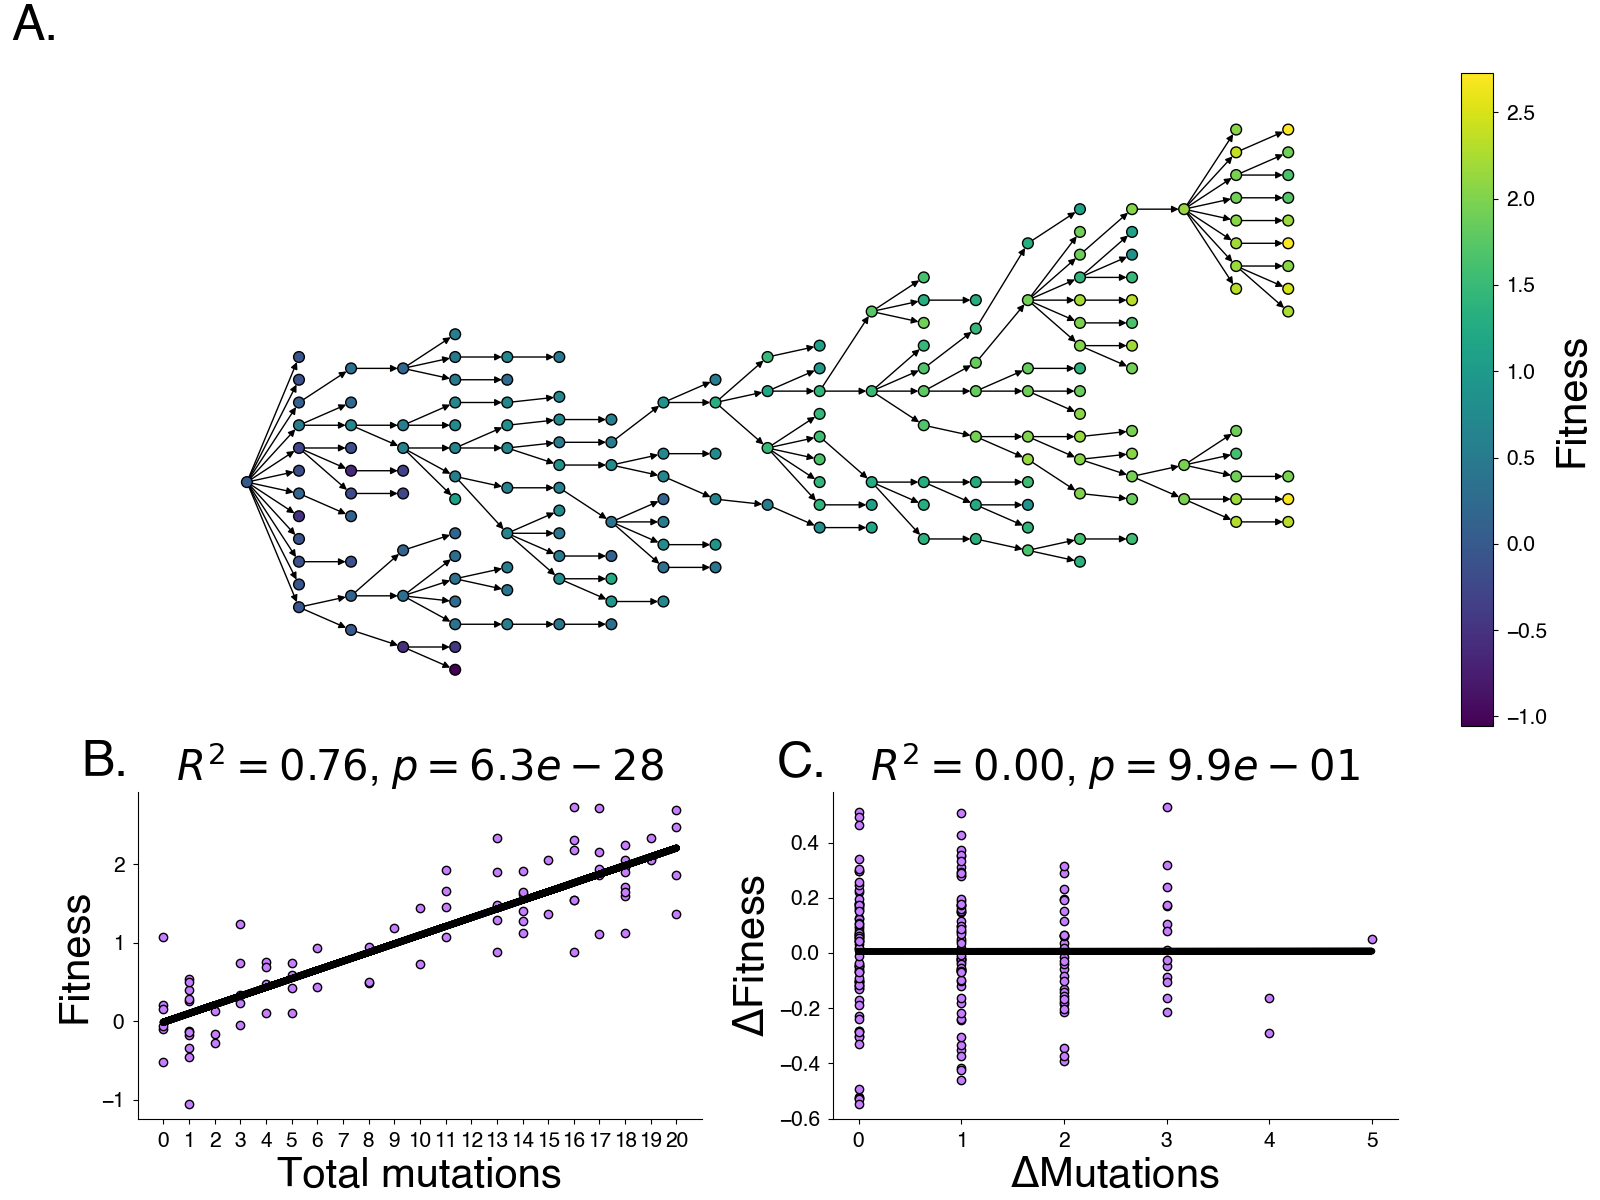
\includegraphics[width=1.0\textwidth]{./figures/synthetic-spurious-correlations.png}
    \caption[\textbf{Shared evolutionary history causes spurious correlations between predictors and fitness.}]{
	\textbf{Shared evolutionary history causes spurious correlations between predictors and fitness.}
	A. A transmission tree simulated with fitness-dependent branching.
	Each branch represents the evolutionary descent of lineages, where fitness evolves through Brownian motion.
	B. Naive regression of tip-level fitness on cumulative mutations.
	This ignores the shared evolutionary history of tips, leading to spurious correlations.
	C. Regression of branch-level innovations (changes in fitness versus changes in mutation counts).
	By analyzing innovations, we account for the shared evolutionary history and isolate the relationship between predictors and fitness, revealing the true lack of direct association.
    }
    \label{fig:shared_history_spurious_correlation}
\end{figure}


\paragraph{Estimating fitness innovations across lineages and clades}

To better understand the variability in fitness changes across SARS-CoV-2 lineages, we apply the innovation idea to an inference model nested within a multinomial logistic regression framework.

This innovation model estimates each lineages' fitness relative to XBB.1.5 and its innovation using the lineage-parent mapping in Fig.~\ref{fig:interplay_phylo_escape_fitness}A.

For this analysis, we use a Normal distribution as a prior for the relative fitness innovations.
We fit this model to XBB.1.5-focused dataset spanning January to November 2023, reflecting the evolutionary dynamics during this period and visualize estimated clade frequencies in Fig.~\ref{fig:interplay_phylo_escape_fitness}C, showing turnover in this period.
These clade frequencies are generated by summing the frequency over all Pango lineages within a clade.

In Fig.~\ref{fig:exploring-fitness-innovations}C, we see that there is clear selection for clades like 23F (EG.5.1) and 24A (JN.1).
Despite this, we see that the overall distribution of innovations is near 0, though it has a wide range with a slight positive skew (Fig.~\ref{fig:exploring-fitness-innovations}B).
This reflects the effect of selection in driving advantageous lineages to higher frequencies, but suggests that both adaptive events and neutral evolutionary processes shaped SARS-CoV-2 evolution in this period.

When aggregated by Nextstrain clade, the fitness innovations present a granular view of the evolutionary trends in SARS-CoV-2 (Fig.~\ref{fig:exploring-fitness-innovations}C).
Generally, clades which appear before 23A (XBB.1.5) such as 22B (BA.5) and 22D (BA.2.75) have a median innovation near 0 which is consistent with neutral evolution.
However, clades following 23A (XBB.1.5.) tend to have positive fitness innovations over average, aligning with their observed growth and dominance during this period. 

This analysis shows that fitness innovations can be used to understand patterns of adaptation within a population or clade.
The variability observed across lineages and clades underscores the role of rare but impactful events in driving lineage success and driving outbreaks.

\begin{figure}[h]
	\centering
	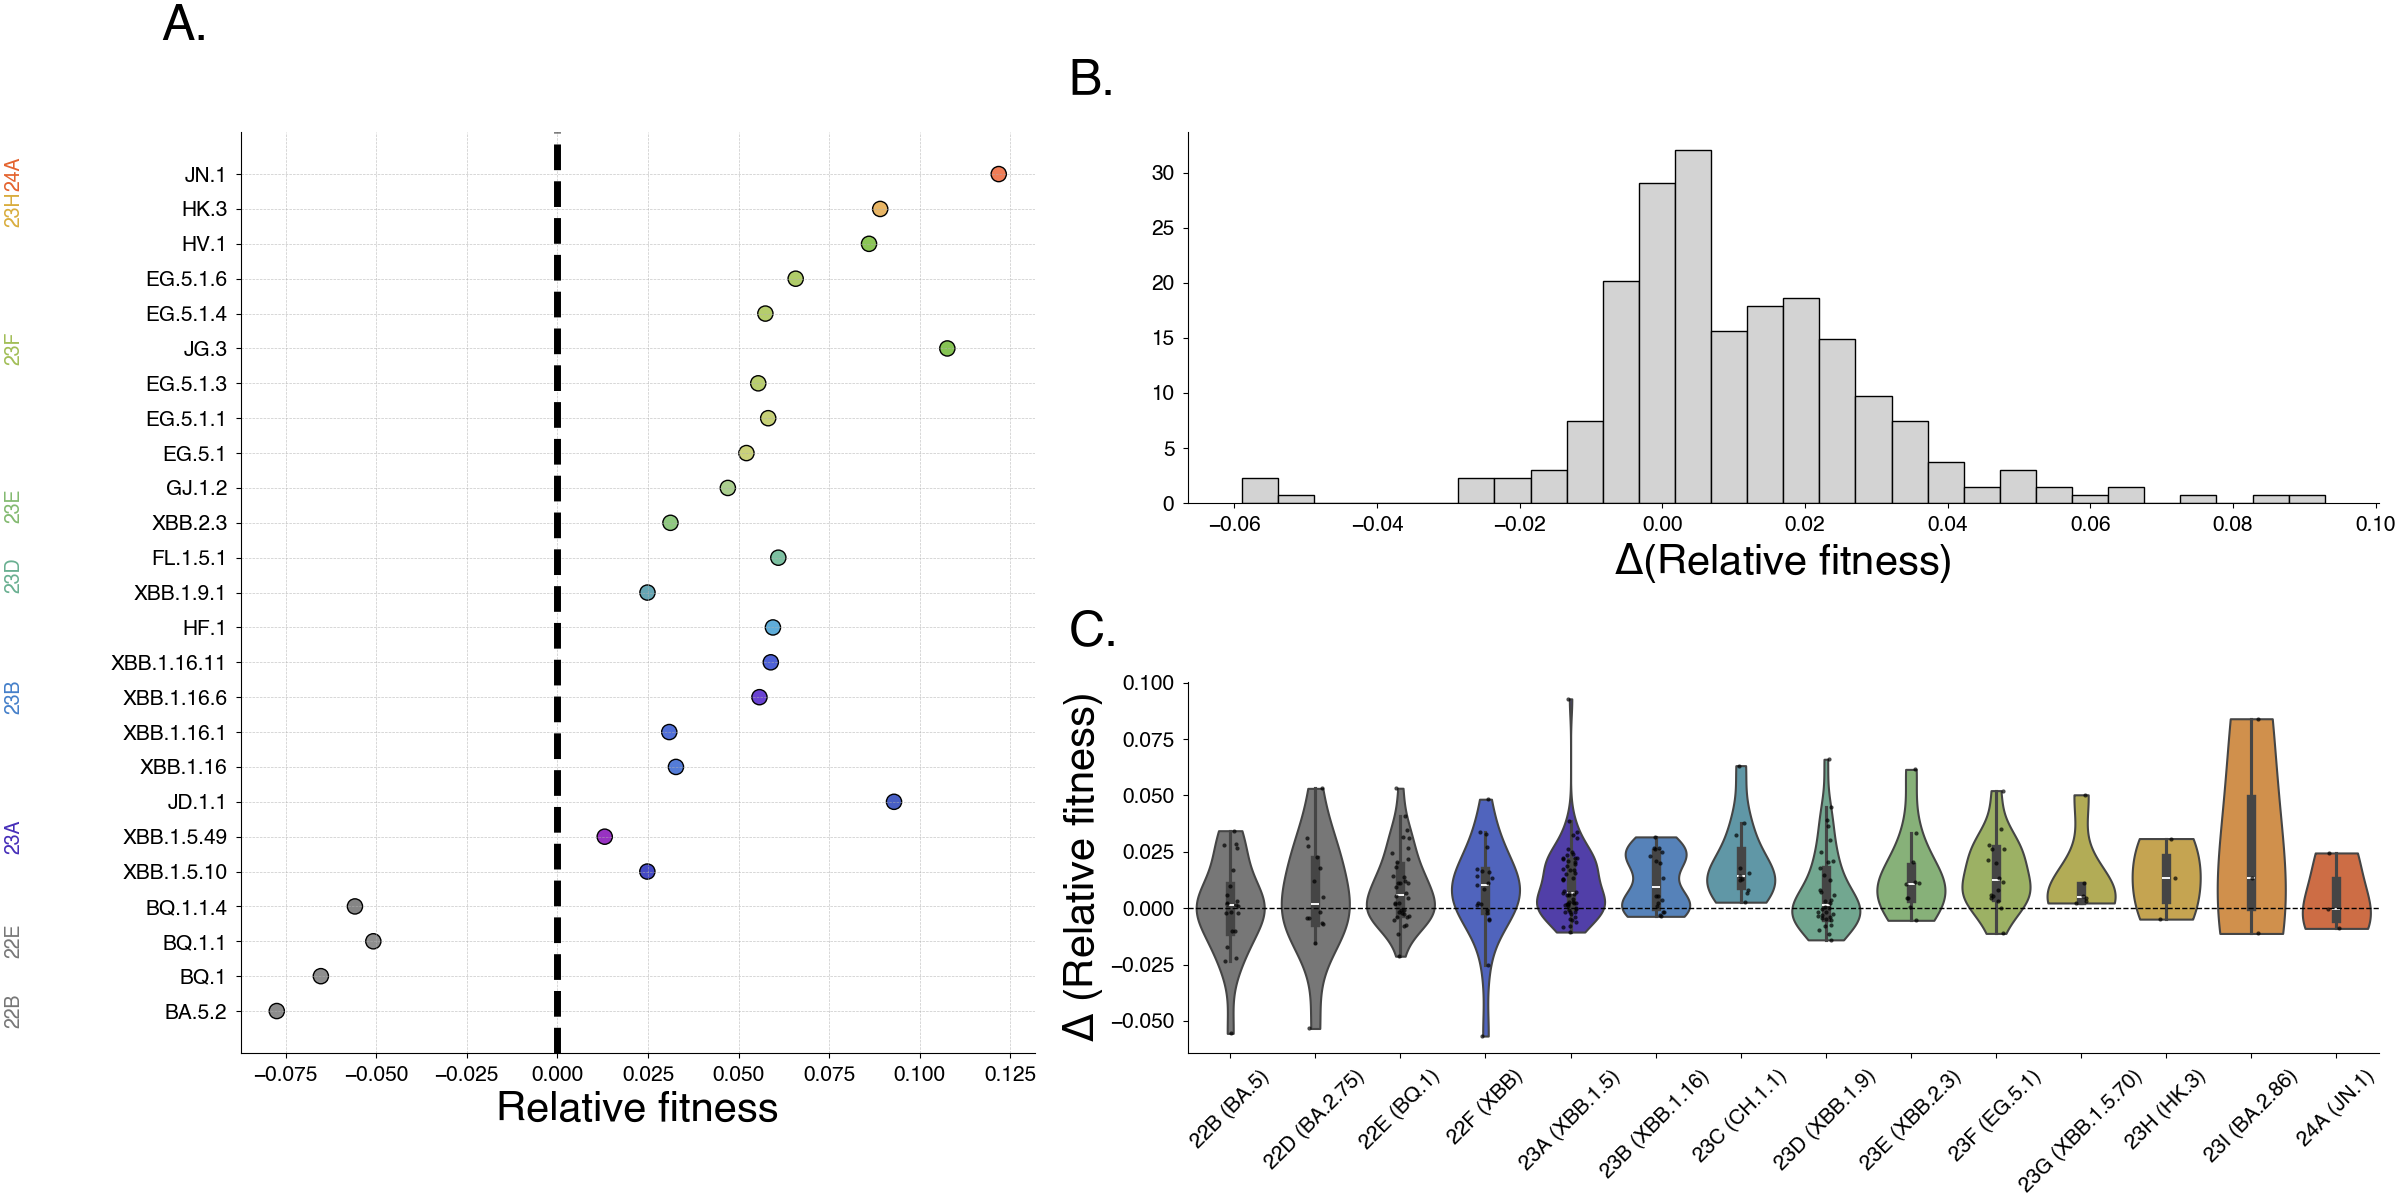
\includegraphics[width=1.0\textwidth]{./figures/exploring-fitness-innovations.png}
	\caption[\textbf{Exploring fitness innovations across SARS-CoV-2 clades.}]{
	    \textbf{Exploring fitness innovations across SARS-CoV-2 clades.}
	    A. Estimated relative fitness for Pango lineages which reach at least 1\% frequency.
	    B. Histogram of overall fitness innovations across all variants.
	    C. Estimated fitness innovations by clade.
	}
	\label{fig:exploring-fitness-innovations}
\end{figure}

\paragraph{Quantifying the relationship between molecular phenotypes and fitness innovations}

To quantify the relationship between molecular phenotypes and fitness innovations, we integrated deep mutational scanning data to predict lineage phenotypes.

For this analysis, we use ``human sera escape relative to XBB.1.5'' and ``ACE2 binding relative to XBB.1.5'' \cite{Dadonaite2023} and ``RBD ACE2 affinity relative to XBB.1.5'', ``RBD expression relative to XBB.1.5'', ``RBD escape relative to XBB.1.5'' \cite{Taylor2023} as phenotypes.

These phenotypes were calculated for each lineage as the sum of all mutation effects relative to XBB.1.5 and lineage-parent differences in these phenotypes were computed to serve as predictors in the innovation-based analyses.

Using the relative fitness innovations estimated previously (Fig.~\ref{fig:explaining-fitness-innovations}A), we use the changes in these phenotypes across parent-child pairs to predict relative fitness with linear regression.
Together, these phenotypes explain a large share of the variance in relative fitness $(R^2=0.79)$, showing the utility of these phenotypes for predicting changes in relative fitness (Fig.~\ref{fig:explaining-fitness-innovations}B).
To understand the contribution of each of these phenotypes to this regression, we estimated the partial $R^2$ of each phenotype (Fig.~\ref{fig:explaining-fitness-innovations}C).
This is a form of the additional variance explained by adding this phenotype to the model.
Using this partial $R^2$ approach shows that RBD yeast-display escape relative to XBB.1.5 explains most of the variance ($R^2_{\text{partial}} = 0.097$).
We repeat this analysis using each predictor individually to predict the relative fitness directly (Fig.~\ref{fig:relative-fitness-single-regressions}) and the relative fitness innovations (Fig.~\ref{fig:relative-fitness-innovations-single-regressions}).

%TODO: Mention other phenotypes.
This analysis shows that molecular phenotypes are able to explain much of the variance of fitness innovations within sample.
Among the phenotypes, RBD yeast-display escape relative to XBB.1.5 contributes the largest unique share to the variance. 
This result emphasizes the role of immune escape and its molecular basis in shaping the success of SARS-CoV-2 lineages.

This suggests these molecular phenotypes may have utility for forecasting the relative fitness of previously unseen SARS-CoV-2 lineages.
% To address this, we implemented a regression-based prior for the relative fitness innovation.
% Using this prior, we can sample relative fitness innovations of a lineage given its phenotype and an in-sample parent lineage.
% This enables direct out-of-sample prediction of relative fitness on unseen lineages exploiting phylogenetic structure and molecular data.

\begin{figure}[h]
	\centering
	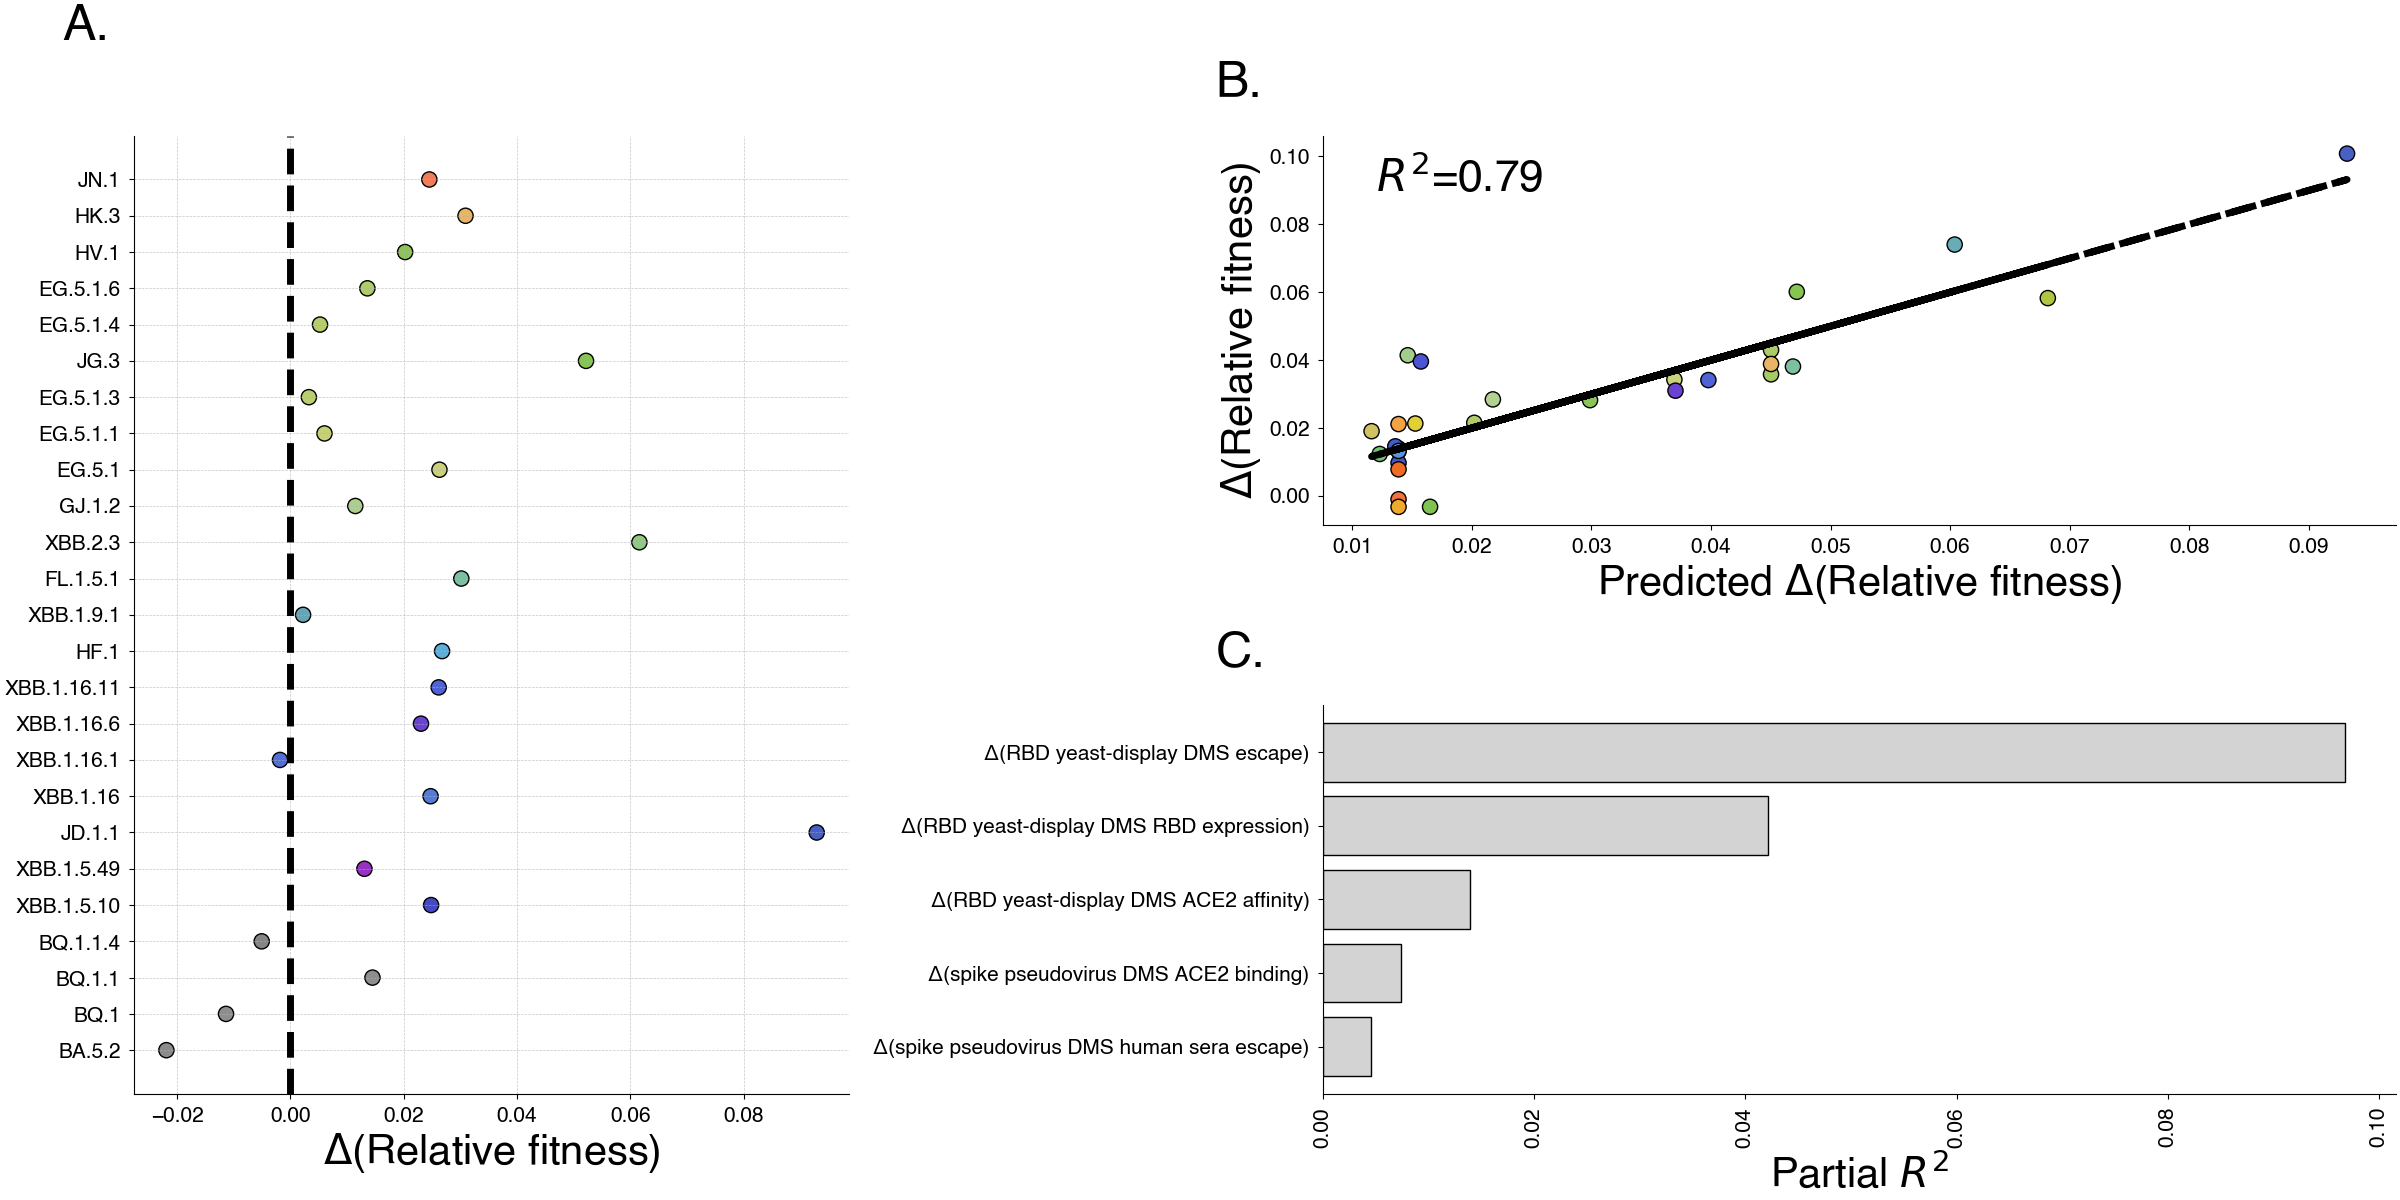
\includegraphics[width=0.95\textwidth]{./figures/explaining-fitness-innovations.png}
	\caption[\textbf{Molecular phenotypes explain fitness innovations.}]{
	    \textbf{Molecular phenotypes explain fitness innovations.}
	    A. Relative fitness innovations for Pango lineages which reach at least 1\% frequency.
	    B. Observed versus predicted relative fitness innovations from the regression model ($R^2 = 0.72$), demonstrating the model’s predictive accuracy.
	    C. Partial $R^2$ values for molecular predictors, illustrating the relative contributions of features such as immune escape, receptor binding, and expression to fitness innovations.
	}
	\label{fig:explaining-fitness-innovations}
\end{figure}

\paragraph{Using molecular phenotypes for out-of-sample relative fitness forecasts}

To assess the predictive utility of molecular phenotypes, we implemented a regression prior for the relative fitness innovation. This approach enables the prediction of fitness innovations for out-of-sample lineages by leveraging their molecular phenotypes and the lineage-parent relationships described previously.
With these predicted fitness innovations, we can then forecast relative fitness using the baseline fitness of its parent (Fig.~\ref{fig:predicting-fitness-with-innovations}C).

We validate that the regression prior fitness model estimates relative fitnesses that are consistent with the relative fitness in the uninformed model (Fig.~\ref{fig:predicting-fitness-with-innovations}A), finding near perfect alignment between the two models ($R^2 = 1.0$).
This suggests that our regression prior fitness model is able to capture both the effect of predictors and estimate the residual between our predictions.

We then sought to validate this model using its predictions for previously unseen variants.
We repeat the same relative fitness analysis, estimating relative fitness using the normal prior model for the 6 months following the end of the original XBB.1.5 data set.
Using all lineages for which we have available phenotypes but were not included in the original data set, we predict their fitness and compare it to the estimated relative fitness in the future data set (Fig.~\ref{fig:predicting-fitness-with-innovations}B).
Our forecasted relative fitness align closely with the future relative fitness though they differ in scale, and we find that our predictions explain a large share of the variance ($R^2 = 0.67$) in future relative fitness and are strongly positive correlated (Spearman's $\rho=0.72$).
This result highlights the ability of the regression-based fitness model to generalize fitness predictions beyond the training set, effectively utilizing molecular phenotypes as predictors.

The ability to predict fitness for previously unseen lineages provides a critical tool for evolutionary forecasting.
By combining molecular phenotypes with the innovation framework, this approach offers a scalable solution for anticipating the success of novel variants in real-time.

\begin{figure}[h]
	\centering
	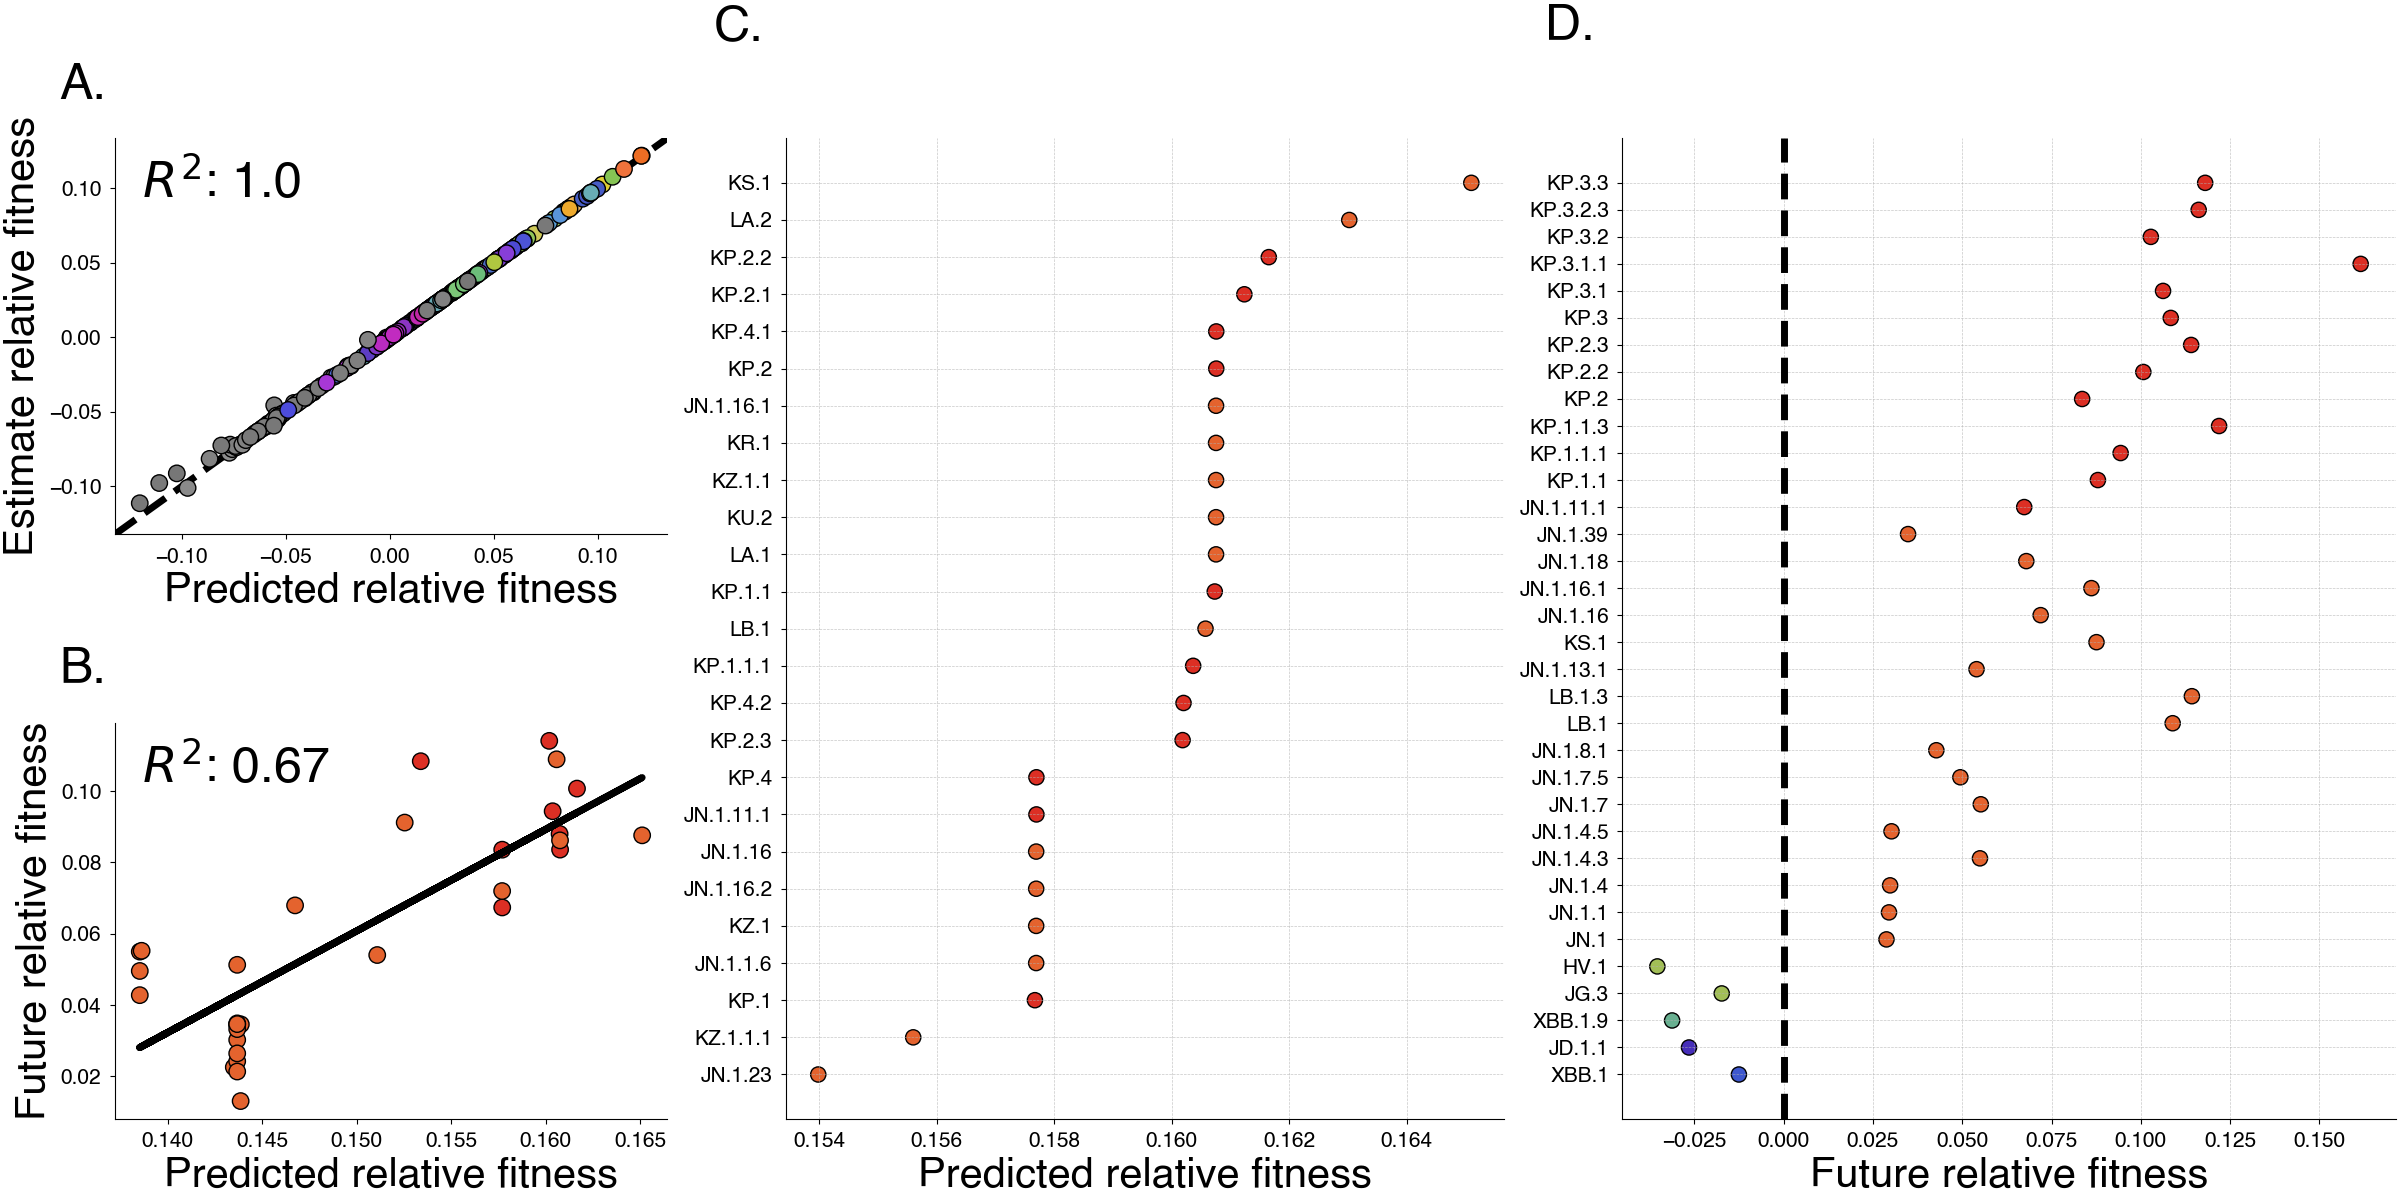
\includegraphics[width=1.0\textwidth]{./figures/predicting-fitness-with-innovations.png}
	\caption[\textbf{Predicting fitness with innovations.}]{
	    \textbf{Predicting fitness with innovations.}
	    A. In-sample validation comparing predicted relative fitness innovations with their estimated values.
	    Predictions were generated using the regression-based prior, incorporating molecular phenotypes as predictors.
	    Points represent individual lineages, with the diagonal dashed line indicating perfect agreement between predicted and estimated values.
	    B. Out-of-sample validation comparing predicted relative fitness innovations with observed values for lineages not included in the training dataset.
	    C. Predicted relative fitness of top 25 lineages.
	    D. Relative fitness lineages achieving at least 2\% frequency, relative fitnesses are estimated with data from the 6 months following training period.
	}
	\label{fig:predicting-fitness-with-innovations}
\end{figure}

\section{Discussion}

This study addresses the challenge of predicting the success of unseen variants in rapidly evolving populations.
By integrating molecular phenotypes with relative fitness, we isolate branch-specific fitness innovations while addressing confounding due to shared ancestry.
Our results suggest that molecular phenotypes, particularly immune escape, are strong predictors of lineage success.
Using a regression-based prior, we extend this approach to enable out-of-sample forecasting of relative fitness, providing a scalable, mechanism-informed framework for understanding and predicting the evolutionary success of emerging variants.

Immune escape emerges as the most significant phenotypic driver of relative fitness, aligning with prior studies suggesting weaker neutralization of emerging variants in hosts with past exposure.
Molecular phenotypes such as ACE2 binding affinity and RBD expression, also contribute though to a lesser extent.
These results emphasize that while immune escape is a primary driver, transmissibility-related traits also play a role in shaping lineage success of SARS-CoV-2.

The ability to predict relative fitness for unseen variants has significant public health implications.
Linking molecular phenotypes to relative fitness enables longer-term forecasts of lineage success, which can inform vaccine strain updates by prioritizing high-fitness lineages for monitoring or use as candidate strains before they reach dominance.

% Further, early identification of high-risk variants has significant public health implications.
% Linking molecular phenotypes to relative fitness can provide longer-term forecasts of lineage success and be used to inform vaccine strain updates by selecting high-fitness lineages for monitoring or as candidate strains before they reach dominance.

Despite its strengths, this approach has several limitations.
The focus on genomic data from the United States may restrict the generalizability to regions with different immune landscapes.
For pathogens like influenza which have greater regional diversity, this consideration becomes extremely important.
Additionally, the assumption that molecular phenotypes independently contribute to fitness innovations may oversimplify the interactions between phenotypic traits, which may motivate more complex, data-informed prior models.

Our framework also relies on the quality and relevance of deep mutational scanning data, which may not fully describe immune escape in all populations due to host-specific differences.
While molecular phenotypes derived from deep mutational scanning are powerful, they may not fully capture complex interactions, such as epistasis.
These limitations also suggest future directions for expanding this framework.

Future work can refine this approach by incorporating larger datasets spanning diverse regions and lineages beyond XBB.1.5, enabling evaluation of its generalizability across varying immune landscapes. Testing additional molecular phenotypes may improve prediction accuracy and reveal novel drivers of fitness.

This study establishes a framework for forecasting relative fitness for SARS-CoV-2 using molecular phenotypes.
By showing the utility of these phenotypes for predicting fitness and enabling out-of-sample forecasts, our approach provides a practical tool for real-time monitoring of emerging variants and informing vaccine strain selection. 
While focused on SARS-CoV-2, the framework can be adapted to study other rapidly evolving pathogens, extending its relevance beyond the current pandemic.
These contributions provide a foundation for advancing long-term evolutionary forecasting and guiding proactive responses to pathogen evolution.

\section{Methods}

\paragraph{Simulation of transmission trees with fitness-weighted offspring}%

To investigate how evolutionary history influences correlations between molecular phenotypes and fitness, we simulated transmission trees using a discrete-generation model.
Each tree begins with a single ancestral lineage at generation 0, initialized with fitness $\lambda_0$.
At each generation $t$, the total number of offspring $O_{t}$ is sampled from a Poisson distribution with mean $bar{N}_t$.
These offspring are then distributed among active lineages $i$ are allocated using a multinomial draw based on fitness-weighted probabilities, so that the offspring by lineage are given by:

\begin{align*}
    O_{i, t} &\sim \text{Multinomial}\left(O_t, p_{i}\right),\\
    p_i &= \frac{\exp(\lambda_i)}{\sum_j \exp(\lambda_j)},
\end{align*}
where $\lambda_i$ is the fitness of lineage $i$.
We assume that the fitness of each offspring evolves from its parent’s fitness according to a Brownian motion process
\begin{equation*}
    \lambda_{\text{offspring}} = \lambda_{\text{parent}} + \psi, \quad \psi \sim \text{Normal}(0, \sigma^2),
\end{equation*}
where $\sigma$ determines the variance in fitness evolution.
Mutations accumulate along branches with their counts drawn from a Poisson distribution with rate $\mu$.

The simulation is run over a fixed number of generations, producing trees where fitness influences both branching structure and phenotype evolution.
These trees are then analyzed to compare naive tip-level regressions with branch-level contrast regressions, providing insight into how shared evolutionary history drives spurious correlations and demonstrating the importance of evolutionary-aware statistical approaches.

\paragraph{Generating sequence counts}%

We prepared sequence count data sets using the Nextstrain-curated SARS-CoV-2 sequence metadata \cite{Hadfield2018} which is created using the GISAID EpiCoV database \cite{khare2021gisaid}.
These sequences were counted according to their annotated Pango lineage \cite{aksamentov2021nextclade}, country of collection, and date of collection to produce sequence counts for each variant, date, and country analyzed.

\paragraph{Multinomial logistic growth}

To estimate relative rates of growth between variants of interest, we fit a multinomial logistic growth model to the sequence count data.
This model can be written as:
\begin{align*}
    f_{t, v} = \frac{\exp(\alpha_{v} + \lambda_{v} t)}{\sum_{u=1}^{V} \exp(\alpha_{u} + \lambda_{u} t)},
\end{align*}
where $\alpha_{V} = \lambda_{V} = 0$.

We can then interpret $\lambda_{v}$ as the relative fitness of variant $v$ relative to variant $V$.
Assuming a fixed generation time $\tau$ additionally allows us to then write the relative $R_{t}$ or growth advantage for variant $v$ over $V$ as $\Delta_{v} = \exp(\lambda_{v}\tau)$.
To fit this model, we use a multinomial likelihood with probabilities defined by the frequencies above, the vector of counts for each variant at time $t$ $S_{t}$, and the total count of sequences at time $t$:

\begin{align*}
    S_{t} \sim \text{Multinomial}(N_{t}, f_{t, \cdot}).
\end{align*}

\paragraph{Mapping variant-parent relationships}%

In order to estimate rough branch-specific relative fitness innovations, we develop a data set mapping variants as parent-child pairs.
For each Pango lineage in our generated sequence counts, we iterate to its parent lineage until the parent lineage is either in the sequence count file or there is no parent present.
If there is no parent present, we simply estimate the variant's relative fitness and growth advantage directly.

\paragraph{Relative fitness innovation model}%

We can extend the previous model for the Multinomial Logistic growth to take into account for evolutionary relationships using the variant-parent lineage mapping generated in the previous section.

This updated model is instead parameterized by the relative fitness difference between variant $v$ and its parent lineages $\psi_{v} = \lambda_{v} - \lambda_{\text{parent}_{v}}$ directly.
Under this parameterization, we can also define the (approximate) growth advantage innovations $\Psi_{v}$ from a variant lineage $v$ to its parent as
\begin{align*}
\Psi_{v} = \frac{\Delta_{v}}{\Delta_{\text{parent}_{v}}} = \exp(\psi_{v} \tau).
\end{align*}

\paragraph{Normal prior model}%

We consider several prior models on the relative fitness innovation $\psi_{v}$.
The most basic of these models is a normal prior on the relative fitness innovations
\begin{align*}
    \psi_{v} = (\lambda_{v} - \lambda_{\text{parent}_{v}}) \sim \text{Normal}(0, \sigma).
\end{align*}
This induces a log normal prior on the growth advantage innovations $\Psi_{v}$.

\paragraph{Regression prior for growth advantage innovations}%

To better explain the variation in relative fitness innovations and enable prediction of relative fitness for new variants given features and their parent lineage, we extend the above prior to be parameterized by various features, so that
\begin{equation}\label{eq:relative_fitness_regression}
    \psi_{v} = (\lambda_{v} - \lambda_{\text{parent}_{v}}) \sim \text{Normal} \left( \sum_{p} \theta_{p} x_{p}, \sigma \right).
\end{equation}

Using this model, we can then predict relative fitnesses and growth advantages out of sample.
For a given out-of-sample variant $v$, we need to only specify its set of predictors $x_{p}$ and its in-sample parent $\text{parent}_v$.
First, we predict its innovation relative to its parent and its total relative fitness by sampling using Equation \ref{eq:relative_fitness_regression} with the estimated $\theta_{p}$.
We can compute the relative fitness of this variant by adding the predicted innovation to the estimated relative fitness of its parent.
This provides an out-of-sample estimate of the relative fitness using a combination of molecular data and our knowledge of the evolutionary history of the population.

% \paragraph{Extending to time-varying growth advantage innovations}%
%
% \begin{align*}
%     \psi_{v,t} &= (\lambda_{v,t} - \lambda_{\text{parent}_{v}, t}) \sim \text{Normal} \left( \sum_{p} \beta_{p} x_{p}, \sigma \right) \\
%     \beta_{p, \cdot} &\sim \text{RandomWalk}(0, \gamma)
% \end{align*}

\paragraph{Generating features for regression prior analysis}%

% TODO: Explain what deep mutational scanning and why RBD is relevant
We use mutation effects estimated using pseudovirus deep mutational scanning and receptor binding domain (RBD) yeast-display deep mutational scanning to predict phenotypes at the level of Pango lineage \cite{Dadonaite2023, Taylor2023}.
The phenotype of each lineage is computed as the sum of all mutation effects relative to XBB.1.5.
This gives us 5 molecular phenotypes: ``spike pseudovirus DMS human sera escape relative to XBB.1.5'', ``spike pseudovirus DMS ACE2 binding relative to XBB.1.5'', ``RBD yeast-display DMS ACE2 affinity relative to XBB.1.5'', ``RBD yeast-display DMS RBD expression relative to XBB.1.'', ``RBD yeast-display DMS escape relative to XBB.1.5''.

We also compute the variant-parent differences in the phenotypes for use as predictors in the innovation-based analyses. 
These variant-parent differences are computed using the variant-parent relationships described above for variants with an existing parent.

\paragraph{Analysing SARS-CoV-2 evolution post-XBB.1.5 emergence.}

To analyze selection in SARS-CoV-2 after the emergence of XBB.1.5, we begin by generating Pango lineage-level sequence counts for the United States between January 1st, 2023 and December 1st, 2023. 
We collapse small lineages which do not meet a count threshold into their parent lineages, forcibly including XBB, XBB.1.5, and XBB.2.
Using these collapsed counts, we generate the variant-parent relationships.
We, then, estimate the relative fitness of each variant and its innovation using these sequence counts and the innovation model with a normal prior on the innovations.

Using these estimated innovations, we fit a standard linear regression between the relative fitness innovation and the molecular phenotype innovations.
To evaluate the contribution of adding individual phenotypes to the relative fitness innovations, we conducted a partial $R^2$ analysis.
We compute the partial $R^2$ for each phenotype as the difference between the $R^2$ of the full model and the $R^2$ of the model without the phenotype of interest.
This approach quantifies the proportion of variance in the dependent variable (relative fitness innovation) explained by each phenotype when adding it to a model that already uses the other phenotypes.

We also estimate the relative fitness of each variant and its innovation to its parent using the regression prior on the innovations with the 5 molecular phenotypes as predictors.
This enables us to make predictors of the phenotype for out of sample lineages as long as we know their parent and their phenotypes.

\subsection*{Acknowledgements}

We gratefully acknowledge all data contributors, i.e. the Authors and their Originating laboratories responsible for obtaining the specimens, and their Submitting laboratories for generating the genetic sequence and metadata and sharing via the GISAID Initiative, on which this research is based.

\subsubsection*{Funding}

This work is supported by NIH NIGMS award R35 GM119774 to TB and a Howard Hughes Medical Institute COVID-19 Collaboration Initiative award to TB.
MF is an ARCS Foundation scholar and was supported by the National Science Foundation Graduate Research Fellowship Program under grant No.\ DGE1762114.
TB is a Howard Hughes Medical Institute Investigator.

\subsubsection*{Competing interests}

All authors declare no competing interests.

\subsubsection*{Data and materials availability}

Molecular phenotype data was provisioned from \href{https://github.com/jbloomlab/SARS2-spike-predictor-phenos}{https://github.com/jbloomlab/SARS2-spike-predictor-phenos} on November 24, 2024.
Sequence data including date and location of collection as well as clade annotation was obtained via the Nextstrain-curated data set that pulls data from GISAID database.
A full list of sequences analyzed with accession numbers, derived data of sequence counts and molecular phenotypes, along with all source code used to analyze this data and produce figures is available via the GitHub repository \href{https://github.com/blab/ncov-escape}{github.com/blab/ncov-escape}.
